\chapter{Modularisation}

\section{Organisation des modules}

\subsection{Répartition sur différents threads}

On isole le moteur de jeu sur un thread qui lui est dédié. 
Le rendu reste sur le thread principal par limitation de la
librairie SFML.
Sont partagées entre ces deux modules la liste des commandes et les 
notification de mise à jour de rendu.
\\\\
La liste de commandes est la seule ressource critique dans le 
fonctionnement et il est nécessaire de empêcher le thread du 
moteur de jeu de modifier la liste de commandes tant que le rendu 
n'est pas effectué. Pour le moment, l'operation de mise à jour dans 
le thread de moteur de jeu est suspendu lorsque l'on réalise une 
opération de rendu.
\\\\
On utilise des notifications de rendu pour savoir lorsqu'une 
opération de rendu est en cours et que l'on ne peut modifier la 
liste des commandes.


\section{Enregistrement et chargement des données}

\subsection{Enregistrement des données}
Le jeu comportant de nombreux éléments aléatoires, on a dû 
réaliser dans un premier temps des fonctions permettant de 
créer une description de ses caractères sous forme de 
string. Puis on a réalisé les fonctions inverses qui 
permettent de définir ses éléments à partir des String ainsi 
obtenues.
\\
On réalise ensuite une description en string des actions à 
l'aide des actions retenues pour l'exécution du retour en 
arrière.
\\
Les différentes string sont ensuite assignées à des tags 
lors de la création du fichier replay.txt de type json.

\subsection{Chargement des données}
Le chargement d'une sauvegarde d'une partie se déroule en 
plusieurs étapes. La première est l'ouverture du fichier 
replay.txt.
\\
On initialise alors le moteur du jeu à l'aide des strings 
correspondant à la carte et aux différents personnages. La 
carte est recréée à l'aide des types de tuiles et des 
différentes hauteurs enregistrées dans le string. Les 
personnages sont enregistrés en fonction de leur classe et 
de leur race, ils sont décrits dans le string dans leur 
ordre de l'équipe, étant donné que le nombre de personnages 
par équipes et le même on a besoin de préciser que le nombre 
d'équipes.
\\
On réalise ensuite les différentes actions de chacun des 
tours enregistrés dans les strings des tours, ainsi puisque 
les personnages ont les mêmes caractéristiques, on n'a pas 
besoin de renseigner des détails comme la vie des 
personnages puisque celle-ci redeviendra la même.


\begin{figure}[H]
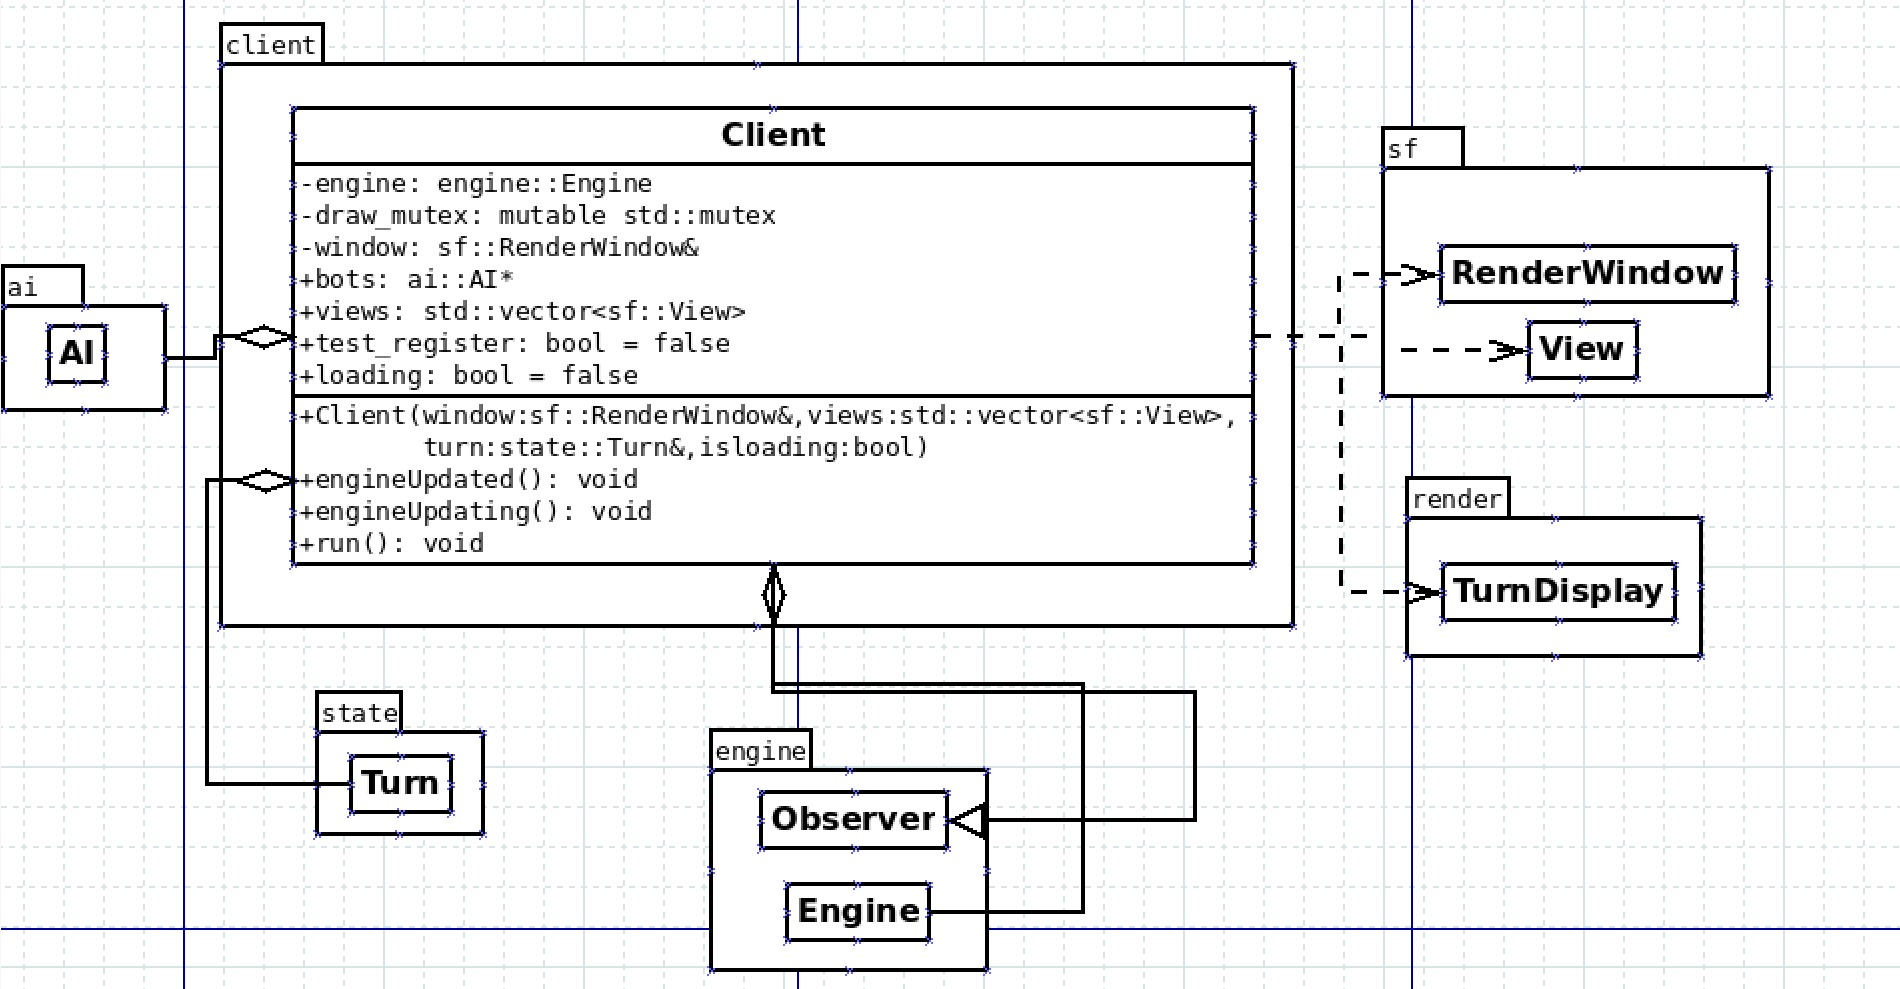
\includegraphics[width=\linewidth]{images/client_dia.png}
\centering
\caption{Aperçu de client.dia}
\label{fig:img6}
\end{figure}
\newpage

\section{Réalisation d'une WebAPI}

\subsection{Description}
On réalise une API REST afin de synchroniser plusieurs 
joueurs sur différentes machine dans une même partie.
\\\\
On réalise dans ce livrable un service dédié à la gestion 
des joueurs dans le lobby. A savoir ajouter un joueur au 
lobby, retirer un joueur du lobby, lister les 
joueurs dans un lobby.
\\\\
Le service player gère les requêtes suivantes:

\begin{itemize}
         \item[•]  \textbf{Requete GET}    /player/<id>\\
Retourne pour l'id corresponant le nom du joueur et le 
booléen inlobby qui est à true quand le joueur n'est pas en 
partie.

         \item[•]  \textbf{Requete GET}    /player/all\\
Retourne la liste complète des joueurs dans le lobby avec le
nom et le booléen inlobby

         \item[•]  \textbf{Requete PUT}    /player\\
On ajoute un joueur à la liste de joueurs du lobby. Le nom 
du joueur est placé dans le body de la requete. 
\\Retourne l'id de ce nouveau joueur dans la liste du 
serveur si le lobby n'est pas plein, sinon retourne un 
message d'erreur indiquant que le lobby est plein.

         \item[•]  \textbf{Requete POST}   /player\\
Analogue à la précédente, la clé-valeur "req":"POST" est 
ajoutée au début du body de la requete. 

         \item[•]  \textbf{Requete DELETE} /player/<id>\\
On retire le joueur correspondant à l'id donné de la liste
de joueurs. 

         \item[•]  \textbf{Requete POST}   /player/<id>\\
Analogue à la précédente, on ajoute la string "disconnect" 
au body. On retire le joueur correspondant à l'id 
donné de la liste de joueurs. 
\end{itemize}


On réalise dans ce livrable un 
service dédié à la gestion 
des commandes. A savoir des 
commandes à la partie, lister les 
commandes de la partie.
\\\\
Le service commandes gère les 
requêtes suivantes:

\begin{itemize}
         \item[•]  \textbf{Requete GET}    /command/<id>\\
Retourne la liste des commandes 
pour le tour pour le numéro id.

         \item[•]  \textbf{Requete GET}    /command/all\\
Retourne la liste des listes de commandes.

         \item[•]  \textbf{Requete POST}    /command\\
On ajoute une liste de commandes à 
la liste des listes de commandes 
de la partie. 
\\Retourne "Done":"Yes" si la commande à bien 
été réussie.
\end{itemize}

On réalise aussi un service dédié 
à la gestion de la génération 
aléatoire au niveau serveur.
Ainsi, le serveur envoie aux 
clients les seeds de la carte et 
des personnages pour que les deux 
joueurs est le même état.
\\Seul la requête GET est 
implémentée pour obtenir les sedds 
des objets générés aléatoirement.

\subsection{Conception Logicielle}

Le diagramme des classes UML C++ pour le serveur est
visible en Figure 6.2.
\\\\
\textbf{Classe Game:} Elle contient la liste de joueurs du 
lobby, 
avec des opérations CRUD sur la liste de joueurs 
(getPlayer,addPlayer,removePlayer,setPlayer)
\\\\
\textbf{Classe Player:} Elle contient les éléments 
caractériques d'un joueur: son ID, son nom et le booleen 
inlobby qui indique si le joueur est en partie ou non. 
\\\\
\textbf{Classe ServiceManager:} Elle est la classe qui 
s'occupe de gérer les services. 
\\La méthode \textbf{registerService}
permet d'enregistrer un service pour qu'il puisse être 
utilisé plus tard lors de la gestion d'une requête.
\\La méthode \textbf{findService} permet 
de trouver le service associé 
à la requête reçue par le serveur: un service étant associé 
à une ressource, il suffit de lire la ressource demandée 
dans l'url pour trouver le service correspondant.
\\La méthode \textbf{queryService} qui va orienter la 
requête vers un type de réponse en fonction 
de la méthode de la requête et 
le contenu de son body pour les requêtes POST.
\\\\
\textbf{Classe Service:} Elle est la classe mère pour
les autres services tels que PlayerService et 
CommandService.
\\\\
\textbf{Classe PlayerService:} Elle gère les requêtes 
présentées plus haut concernant l'ajout, la modification et 
la supression de joueurs dans la liste de joueurs du lobby. 
\\\\
\textbf{Classe CommandsService:} Elle gère les requêtes 
présentées plus haut concernant 
l'ajout et l'obtention des 
commandes de la partie. 
\\\\
\textbf{Classe InitializeService:} 
Elle gère la requête d'obtention 
des seeds correspondant aux 
éléments générés aléatoirement de 
la partie. 
\\\\
\textbf{Classe ServiceException:} Elle permet de gérer 
les exceptions et de retourner le message d'erreur.
\\\\
\textbf{Classe HttpStatus:} Elle est l'énumération des codes HTTP, utilisé dans les réponses aux requêtes. 

\begin{figure}[H]
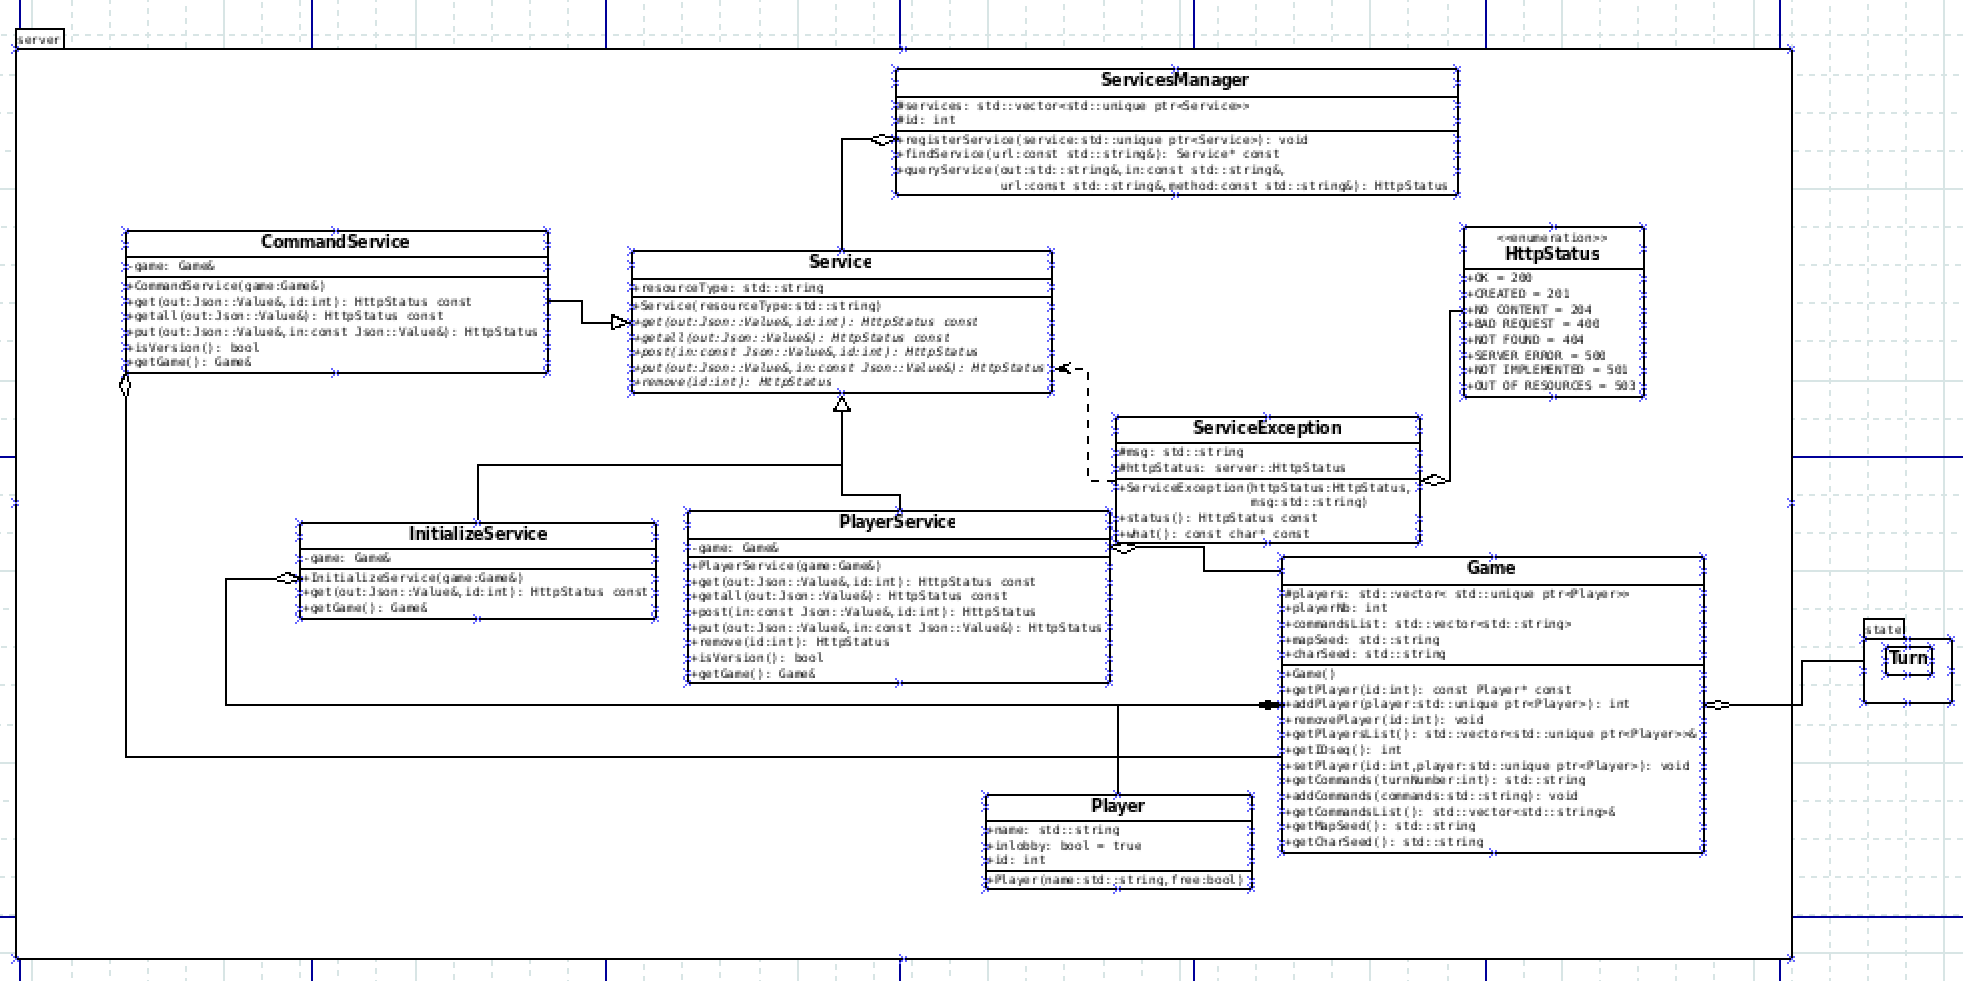
\includegraphics[width=\linewidth]{images/server_dia.png}
\centering
\caption{Aperçu de server.dia}
\label{fig:img6}
\end{figure}
\newpage